\section{Introduction}
  The Fourier Transform (FT) is a function that maps a function in the spacial domain, to the frequency domain.
This is a very useful technique in image processing, because many types of the noise encountered in digital images
is periodic.  This means that if the frequency of the noise ($\frac{1}{\textup{period}}$) is known then it can
simply be removed in the frequency domain.  Working in the frequency domain also has the benefit of easily filtering
out other undesired frequencies.  High frequencies, such as edges can be softened by filtering out higher frequencies,
similarly the edges can be sharped by filtering out the lower frequencies.  Another important property of the
FT is that it can be inverted.  This means that the original equation can be derived by applying the inverse
FT to the the FT of the original function.

  The 2D continuous Fourier Transform is defined in Eq.~\ref{eq:ft} and~\ref{eq:ift}, these equation can be adapted to the
discrete case as Eq.~\ref{eq:dft} and~\ref{eq:idft} shows, this is called the discrete Fourier Transform (DFT).  While the
continuous Fourier Transform has uses in many other fields of
signal processing, it is not relevant, except for deriving the DFT in this work because digital images exist only
as discrete functions.  In Eq.~\ref{eq:dft} and~\ref{eq:idft}, $M$ and $N$ stand for the height and width
of the image.  It is important to notice that if these values are equal the only difference in between the forward and
reverse DFT is the sign of the exponent.  This is a property that simplifies implementation of the function because
the function only needs to be implemented once with a flag to denote the sign of the exponent.

  Using these definitions it can also be shown that the multiplication of two functions in the frequency domain is
equivalent to convolution in the spacial domain.  Although applying this property using Eq.~\ref{eq:dft} and~\ref{eq:idft}
to compute the DFT, the complexity is no better than convolution in the spacial domain, however using a technique known as
the Fast Fourier Transform (FFT) this operation becomes much more efficient.

\begin{equation}
  \label{eq:ft}
  \Im(f(x,y))=F(u,v)=\int_{-\infty}^{\infty} \int_{-\infty}^{\infty} f(x,y)e^{-j2\pi(ux+vy)} dx dy
\end{equation}

\begin{equation}
  \label{eq:ift}
  \Im^{-1}(F(u,v))=f(x,y)=\int_{-\infty}^{\infty} \int_{-\infty}^{\infty} F(u,v)e^{-j2\pi(ux+vy)} du dv
\end{equation}

\begin{equation}
  \label{eq:dft}
  \Im(f(x,y))=F(u,v)=\frac{1}{M} \sum_{x=0}^{M-1} \sum_{y=0}^{N-1} f(x,y) e^{-j2 \pi ( \frac{ux}{M} + \frac{vy}{N} )}
\end{equation}

\begin{equation}
  \label{eq:idft}
  \Im^{-1}(F(u,v))=f(x,y)=\frac{1}{N} \sum_{u=0}^{M-1} \sum_{v=0}^{N-1} F(u,v) e^{j2 \pi ( \frac{ux}{M} + \frac{vy}{N} )}
\end{equation}

\section{Implementation}
  For this project, the FFT function from the Numerical Recipes book was used.  By using the separability of the 2D DFT,
this was achieved by simply applying the FFT on all the rows of an image, followed by applying on all the columns.  For
viewing and editing purposes, the image was shifted by negating every other pixel in the image before applying this transformation.
This effectively shifted the image by half, making it easier to view and also easier to modify.

  The first experiment required that the 2D FFT function be tested on a 32x32 pixel rectangle located in the center of a 512x512 pixel
image.  Once the FFT was calculated for the image, it was normalized to a logarithmic scale between 0 and 255 to be displayed.

  The second experiment was a bit more complex, as it required that the FFT of the image be found and then modified.  After calculating
the FFT of the noisy boy image, the four strongest pixels needed to be replaced with the average of their neighbors.  This was done by
searching the image and building a list of four pixels with the highest magnitude.  Any pixel within 5\% of the center of the image was
ignored to prevent center pixels from being removed (the reason for this is explained in the Results section).  After finding these pixels
and replacing with the average of the neighbors the inverse FFT was found and saved as the resulting image.

  In an attempt to remove the noise in the spacial domain, various Gaussian kernel were constructed and filtered across the image.  The
kernel was calculated using a variance of approximately $1$.  Then the values in the kernel were divided by the sum of values to make
sure all the values summed to 1.  This ensured that the image would not be dimmed or brightened by the filter.  A total of four filters
were tested on the image, those being a 5x5, 7x7, 15x15, and 25x25.

\section{Results}

  The results of taking the FFT of the rectangle image verified that the FFT worked as predicted and returned a $sinc$ function.  This
could be shown by taking the 2D FFT of a step function with a finite range.

  By removing the four pixels with the greatest magnitude the four most prominent frequencies were removed from the image.  By looking
  at the image the most prominent frequencies appear to obviously be the cosine noise that has been added to the image.  The reason that
  the center pixels must be ignored is because the very low frequencies such as flat surfaces actually take up the majority of the image
  which means they are the most prominent frequencies, if they were removed the image would be sharpened, and many of the important features
  would be lost.

  The results of the Gaussian filtering in the spacial domain did not work nearly as well as directly modifying the frequency domain.  By
  looking at the results in the Images section, it seems that the noise is not even removed after using a 25x25 filter, at which point
  so much of the image quality has been lost that it would be pointless to blur any more.  This shows that working in the frequency 
  domain does have some great benefits over the spacial domain because it would be nearly impossible to remove the noise there, while
  it was very easy to do so in the frequency domain (modifying only four pixels!).

\newpage

\section{Source Code}
  \subsection{funcs.h}
    \lstinputlisting{../funcs.h}
  \subsection{main.cc}
    \lstinputlisting{../main.cc}
%  \subsection{image.h}
%    \lstinputlisting{../image.h}
\section{Images}
  %\begin{figure}[hbt]
%  \centering
%  \label{fig:}
%  \subfigure[CAP]{
%    \includegraphics[width=0.4\textwidth]{}
%  }
%  \caption{}
%\end{figure}

~\vfill
\newcolumntype{T}{>{\centering\arraybackslash} m{0.10\textwidth} }
\newcolumntype{S}{>{\centering\arraybackslash} m{0.135\textwidth} }
\begin{tabular}{ T S @{} S @{} S @{} S @{} S @{} S }
  \centering
  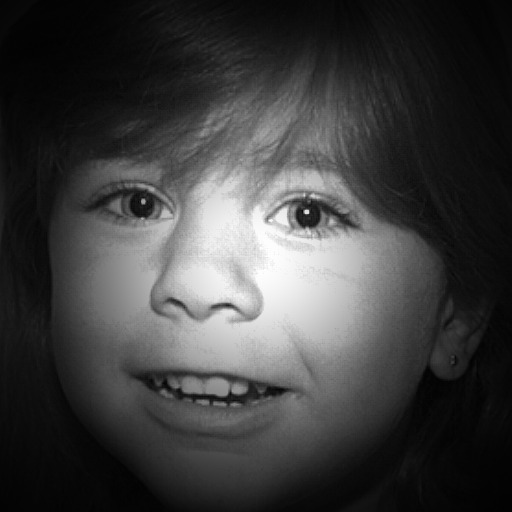
\includegraphics[width=0.1\textwidth]{../images/girl}
  & $\gamma_L=0.2$ & $\gamma_L=0.3$ & $\gamma_L=0.4$ & $\gamma_L=0.5$ & $\gamma_L=0.6$ & $\gamma_L=0.7$ \\
  $\gamma_H=1.2$
  & 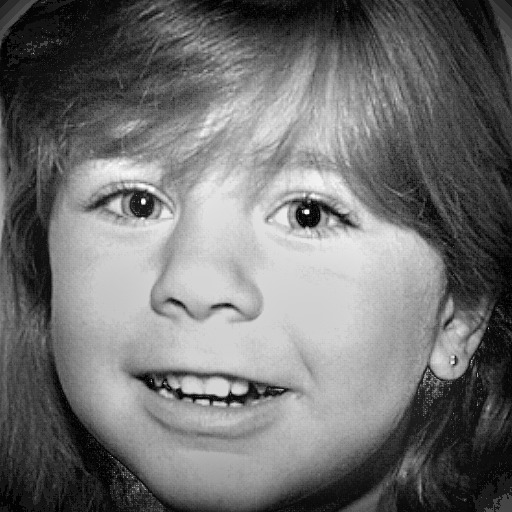
\includegraphics[width=0.135\textwidth]{../images/girl_2_12}
  & 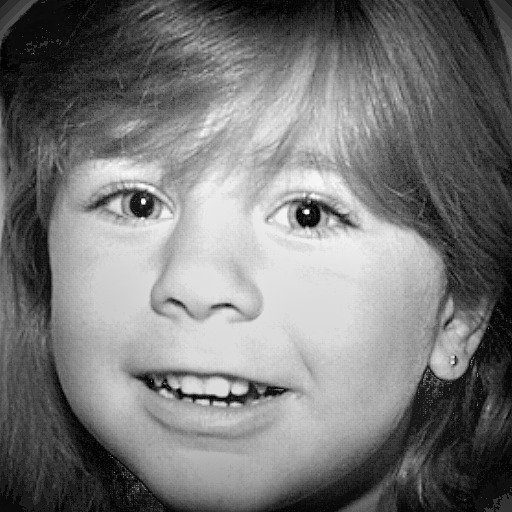
\includegraphics[width=0.135\textwidth]{../images/girl_3_12}
  & 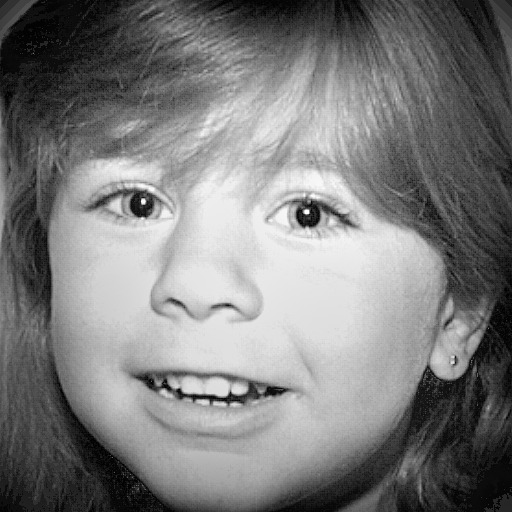
\includegraphics[width=0.135\textwidth]{../images/girl_4_12}
  & 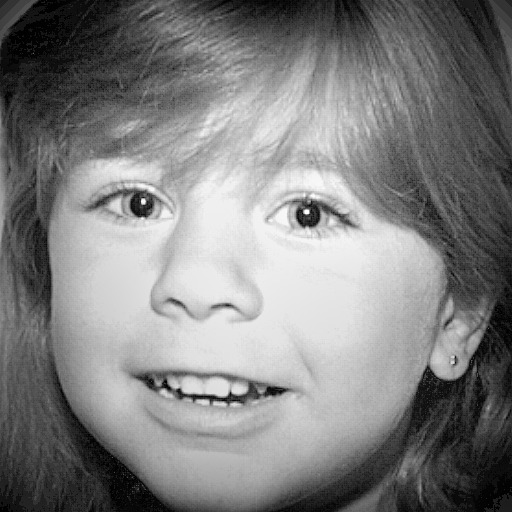
\includegraphics[width=0.135\textwidth]{../images/girl_5_12}
  & 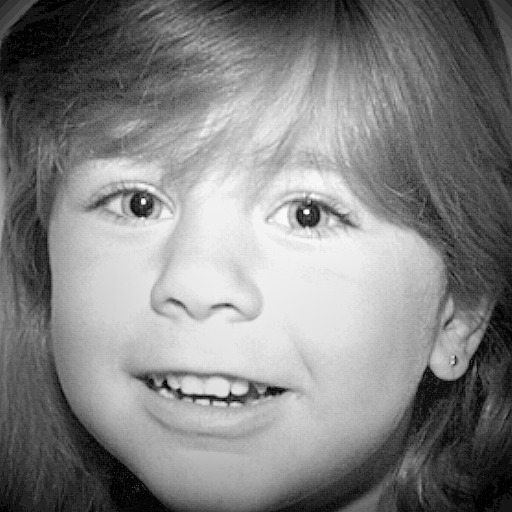
\includegraphics[width=0.135\textwidth]{../images/girl_6_12}
  & 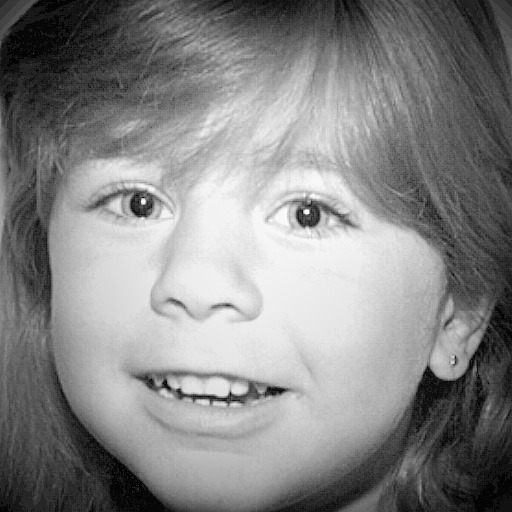
\includegraphics[width=0.135\textwidth]{../images/girl_7_12} \\ [-4pt]
  $\gamma_H=1.3$
  & 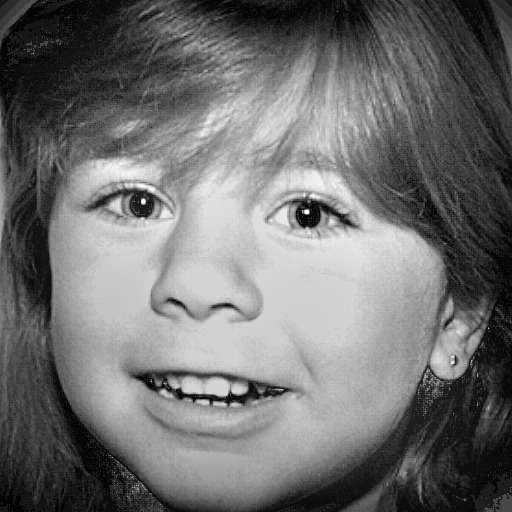
\includegraphics[width=0.135\textwidth]{../images/girl_2_13}
  & 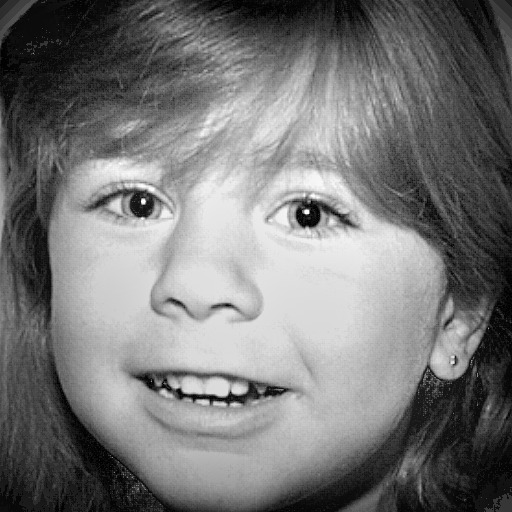
\includegraphics[width=0.135\textwidth]{../images/girl_3_13}
  & 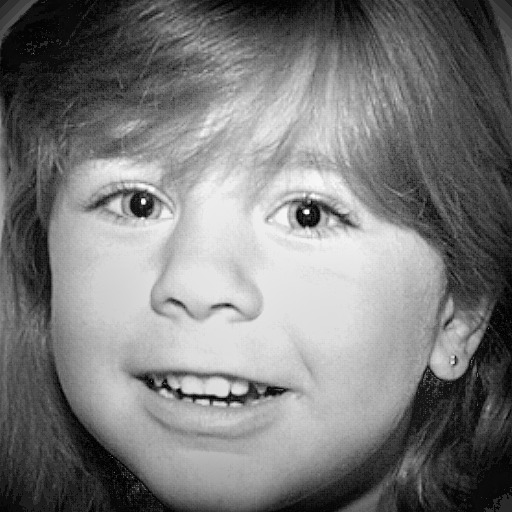
\includegraphics[width=0.135\textwidth]{../images/girl_4_13}
  & 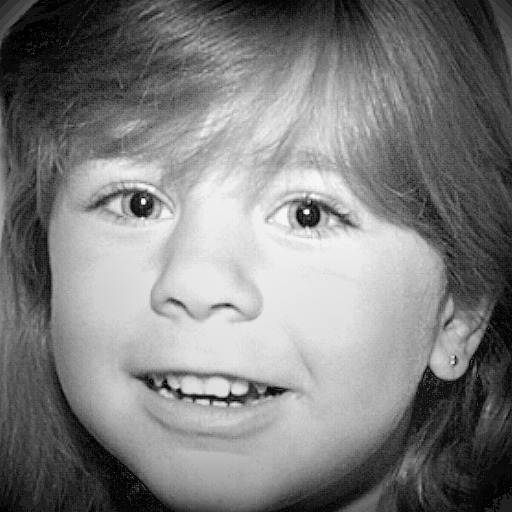
\includegraphics[width=0.135\textwidth]{../images/girl_5_13}
  & 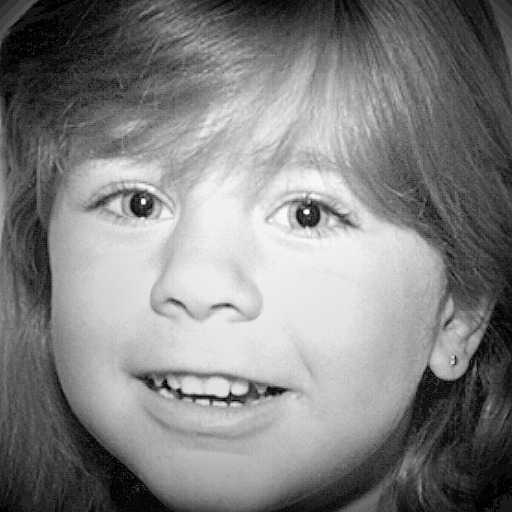
\includegraphics[width=0.135\textwidth]{../images/girl_6_13}
  & 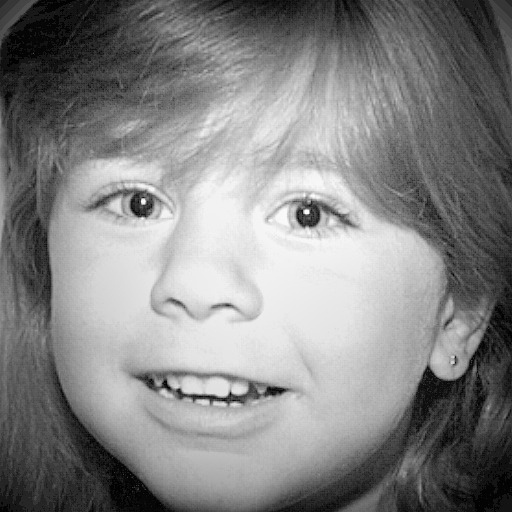
\includegraphics[width=0.135\textwidth]{../images/girl_7_13} \\ [-4pt]
  $\gamma_H=1.4$
  & 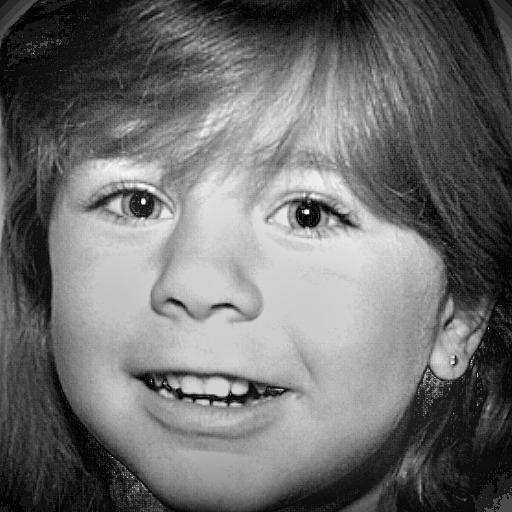
\includegraphics[width=0.135\textwidth]{../images/girl_2_14}
  & 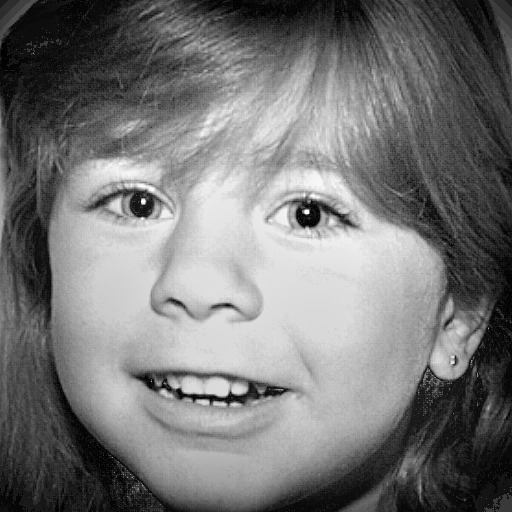
\includegraphics[width=0.135\textwidth]{../images/girl_3_14}
  & 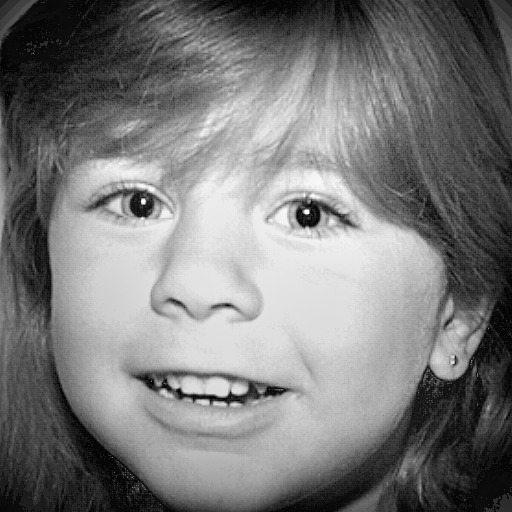
\includegraphics[width=0.135\textwidth]{../images/girl_4_14}
  & 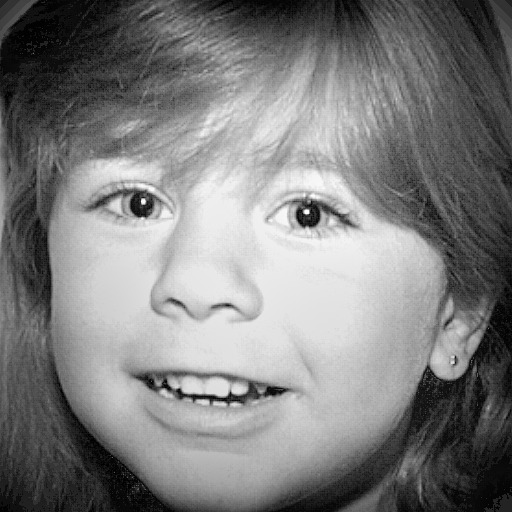
\includegraphics[width=0.135\textwidth]{../images/girl_5_14}
  & 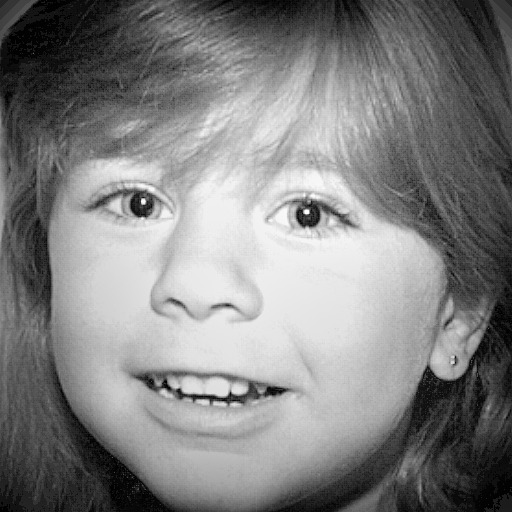
\includegraphics[width=0.135\textwidth]{../images/girl_6_14}
  & 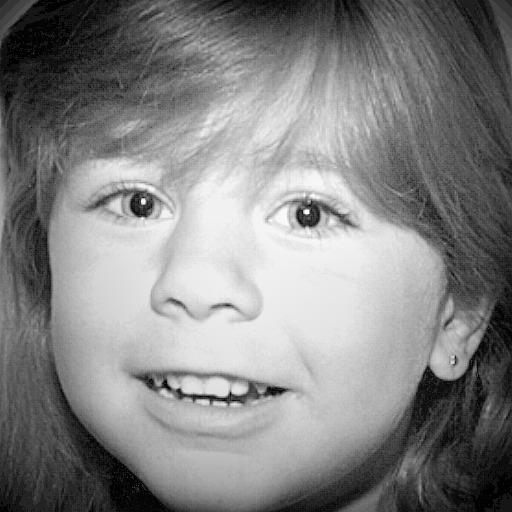
\includegraphics[width=0.135\textwidth]{../images/girl_7_14} \\ [-4pt]
  $\gamma_H=1.5$
  & 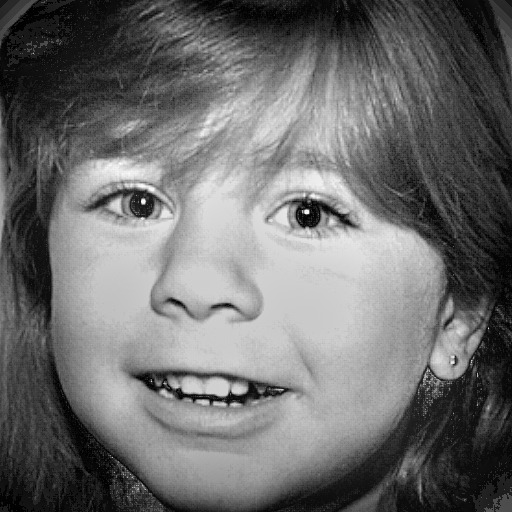
\includegraphics[width=0.135\textwidth]{../images/girl_2_15}
  & 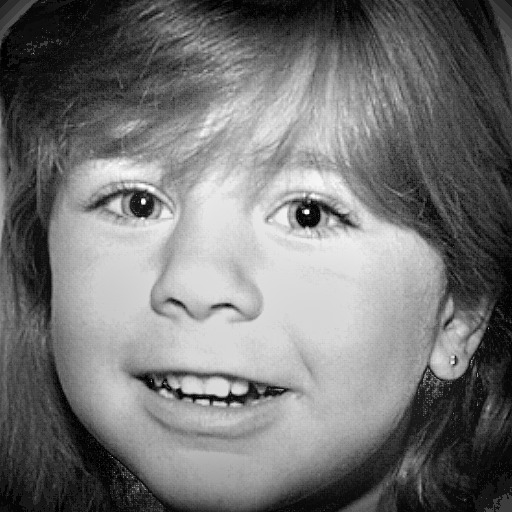
\includegraphics[width=0.135\textwidth]{../images/girl_3_15}
  & 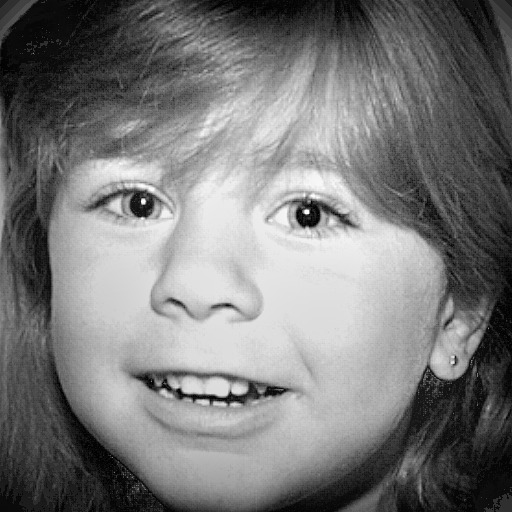
\includegraphics[width=0.135\textwidth]{../images/girl_4_15}
  & 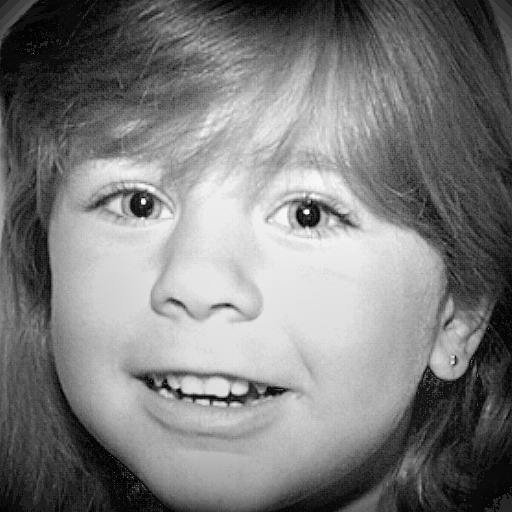
\includegraphics[width=0.135\textwidth]{../images/girl_5_15}
  & 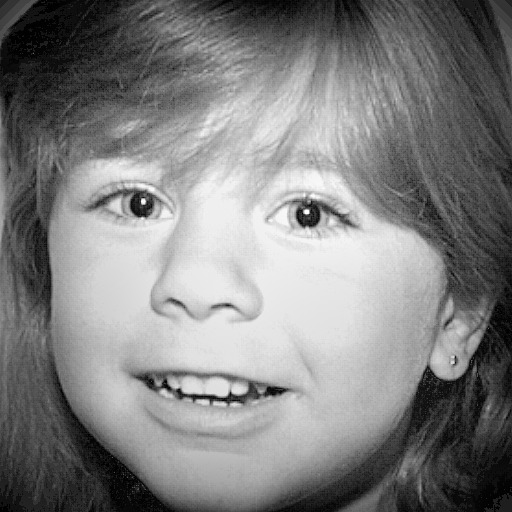
\includegraphics[width=0.135\textwidth]{../images/girl_6_15}
  & 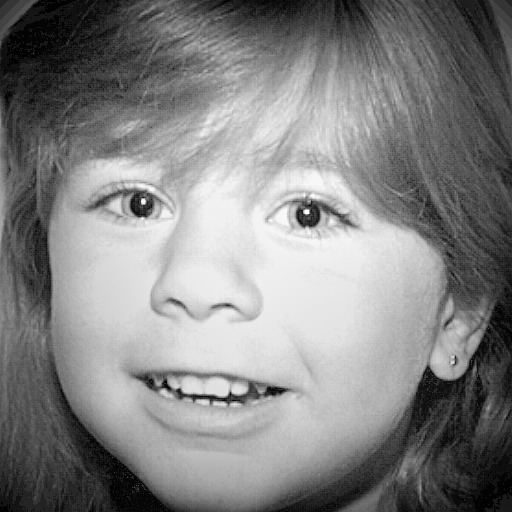
\includegraphics[width=0.135\textwidth]{../images/girl_7_15} \\ [-4pt]
  $\gamma_H=1.6$
  & 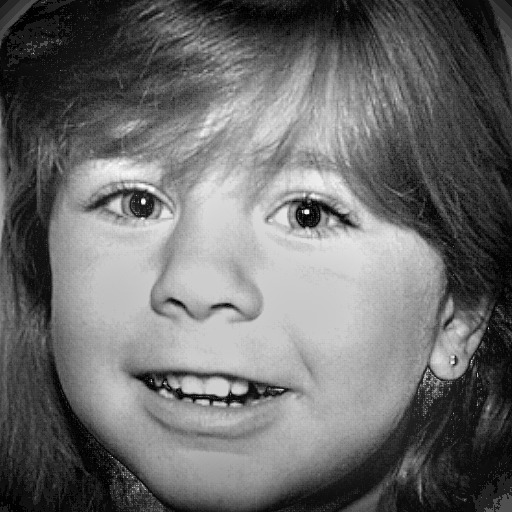
\includegraphics[width=0.135\textwidth]{../images/girl_2_16}
  & 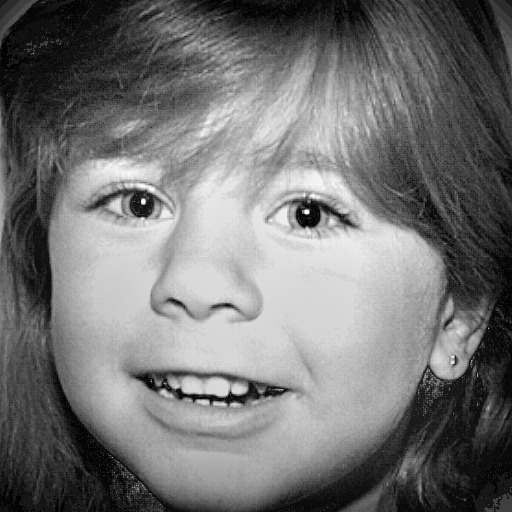
\includegraphics[width=0.135\textwidth]{../images/girl_3_16}
  & 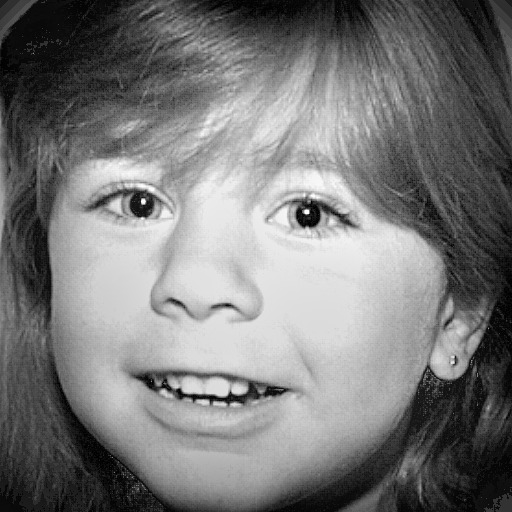
\includegraphics[width=0.135\textwidth]{../images/girl_4_16}
  & 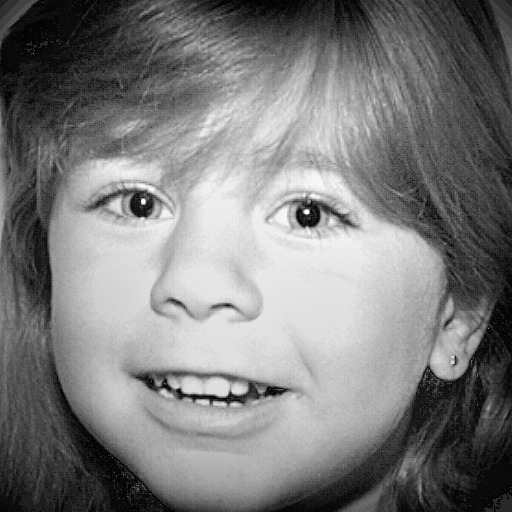
\includegraphics[width=0.135\textwidth]{../images/girl_5_16}
  & 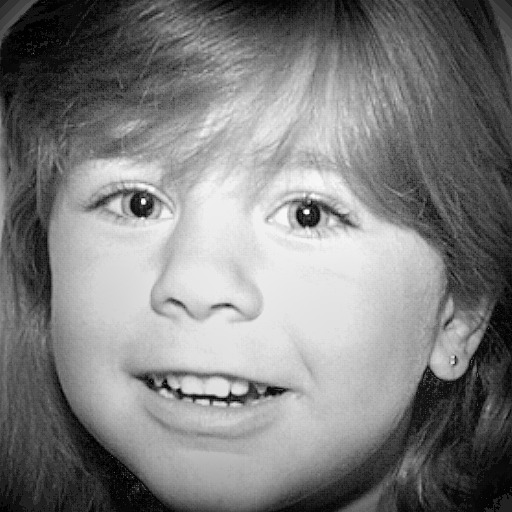
\includegraphics[width=0.135\textwidth]{../images/girl_6_16}
  & 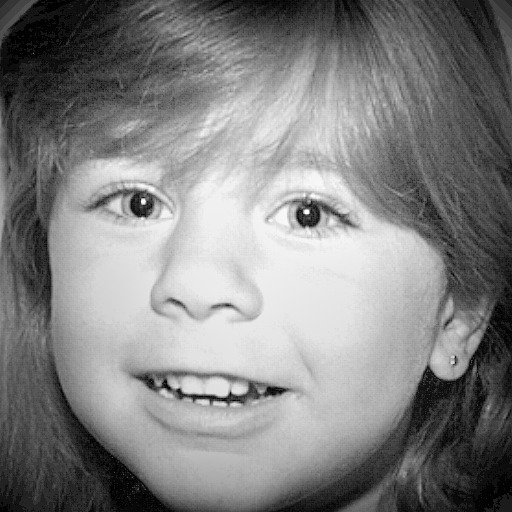
\includegraphics[width=0.135\textwidth]{../images/girl_7_16} \\ [-4pt]
  $\gamma_H=1.7$
  & 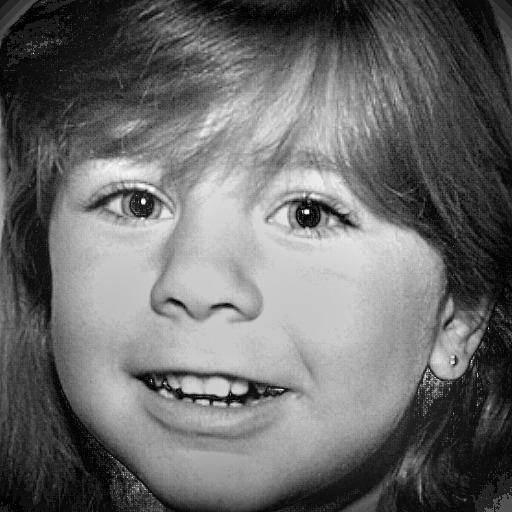
\includegraphics[width=0.135\textwidth]{../images/girl_2_17}
  & 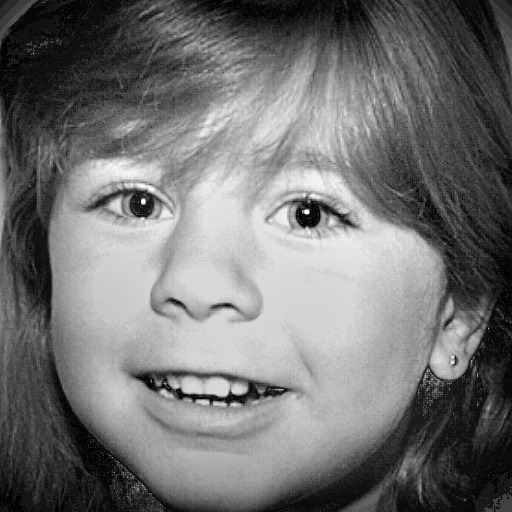
\includegraphics[width=0.135\textwidth]{../images/girl_3_17}
  & 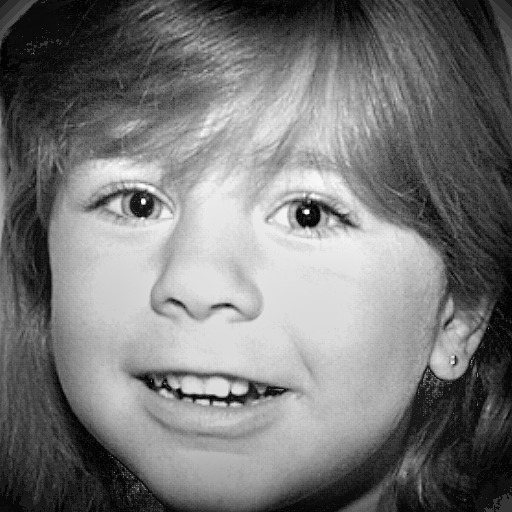
\includegraphics[width=0.135\textwidth]{../images/girl_4_17}
  & 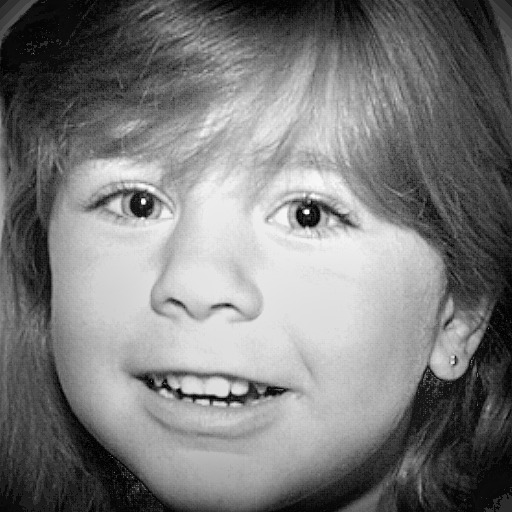
\includegraphics[width=0.135\textwidth]{../images/girl_5_17}
  & 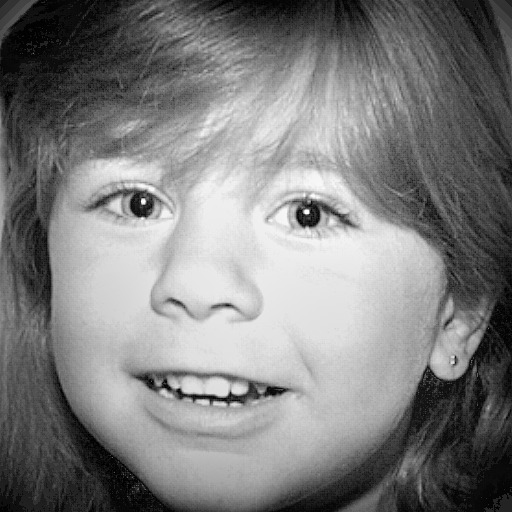
\includegraphics[width=0.135\textwidth]{../images/girl_6_17}
  & 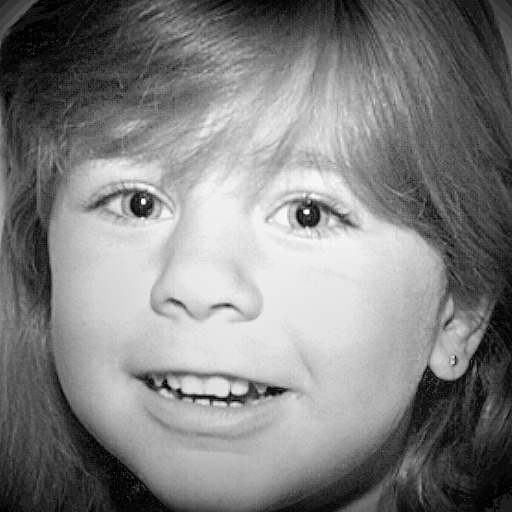
\includegraphics[width=0.135\textwidth]{../images/girl_7_17} \\ [-4pt]

  
\end{tabular}
\vfill

